\documentclass{report}

\usepackage[french]{babel}
\usepackage[utf8]{inputenc}
\usepackage[T1]{fontenc}
\usepackage{listings, lstautogobble}
\usepackage{graphicx}
\usepackage{geometry}
\usepackage[strings]{underscore}

\lstset{
	language=Python,
	frame=single,
	numbers=left,
	tabsize=4,
    autogobble=true,
	showstringspaces=false
}

\geometry{
	hmargin=2.5cm,
	vmargin=1.5cm
}

\title{Implémentation de \\l'algorithme de Dijkstra et sa variante A* \\en Python 3 et Tkinter}
\author{\textsc{Boisnier} Thomas}
\date{4 avril 2018}

\begin{document}

% Page de garde
\maketitle

% Sommaire
\renewcommand{\contentsname}{Sommaire}
\tableofcontents

% Content

% Le projet donne lieu à la rédaction d’un rapport qui devra présenter le projet, expliquer les algorithmes, décrire la structure de l’application et dégager les différents concepts que sa réalisation a nécessité.

\chapter*{Introduction}
\addcontentsline{toc}{chapter}{Introduction}
Au cours de ce document, nous allons examiner comment nous avons implémenter l'algorithme de Dijkstra, ainsi que sa variante A* \cite{Wiki} \cite{A*} afin d'avoir un rendu graphique à la fois simple et ludique.
Nous utiliserons pour cela le langage Python 3 \cite{Python} avec Tkinter \cite{Tkinter} pour tout ce que est de l'interface utilisateur.
Le tout sera basé sur l'implémentation effectué par Xueqiao (Joe) Xu \cite{PathFinding}.

\chapter{Algorithmes}
	\section{Principe}
	L'algorithme de Dijkstra (de son inventeur Edsger Dijkstra) ainsi que sa variante, le A*, sont utilisés (à l'origine) pour rechercher le plus court chemin entre 2 points (itinéraires routiers, etc).\\
	
	Pour se faire, les algorithmes utilisent plusieurs éléments :
	\begin{itemize}
		\item[•] un point de départ
		\item[•] un point d'arrivé
		\item[•] un calcul de distance
		\item[•] une heuristique (uniquement pour A*)
		\item[•] une liste qui contiendra les points visités
		\item[•] une file à priorité qui contiendra les points accessibles (tri croissant du coût global : distance + heuristique)
	\end{itemize}
	\vspace{4mm}
	On commence au point de départ choisi. 
	On estime ensuite la distance qui sépare ce point du point d'arrivé voulu ainsi que son heuristique, puis on l'ajoute à la file à priorité.
	
Les algorithmes retirent le premier point de la file d'attente prioritaire (dû au fonctionnement d'une file d'attente, le point au coût global le plus bas est retiré en premier). Si la file d'attente est vide, il n'y a aucun chemin du point de départ au point d'arrivé, ce qui interrompt l'algorithme. Si le point retenu est le point d'arrivée, les algorithmes reconstruisent le chemin complet et s'arrête.

Si le point retenu n'est pas le point d'arrivé, on ajoute tous les points accessibles à la file a priorité (en calculant leurs coût global à partir du point retenu).

Les algorithmes maintiennent également la liste de points qui ont été visités (couramment appelée "closed list"). Si un point nouvellement produit est déjà dans cette liste avec un coût égal ou inférieur, aucune opération n'est faite sur ce point.

Après, l'évaluation du coût du nouveau point au point d'arrivé, ce nouveau point est alors ajouté à la liste d'attente prioritaire, à moins qu'un point identique dans cette liste ne possède déjà une coût inférieure ou égale.

Une fois les trois étapes ci-dessus réalisées pour chaque nouveau point accessible, le point original pris de la file d'attente prioritaire est ajouté à la liste des points vérifiés. Le prochain point est alors retiré de la file d'attente prioritaire et le processus recommence.
	
	\newpage
	\section{Heuristiques}
	L'algorithme A* nécessite une heuristique, on va donc en définir 4, de sorte que $node$ soit le point actuel, $target$ soit le point d'arrivée, et $m\_x$, $m\_y$ les coordonées en x et en y des points.\\
	
	\begin{itemize}
		\item[•] Manhattan : 
			\begin{lstlisting}
				def manhattan(node, target):
					dx = abs(node.m_x - target.m_x)
					dy = abs(node.m_y - target.m_y)
					
					return dx + dy
            \end{lstlisting}
		\item[•] Euclidien : 
			\begin{lstlisting}
				def euclidean(node, target):
				    dx = node.m_x - target.m_x
				    dy = node.m_y - target.m_y
				    
				    return sqrt(dx * dx + dy * dy)
            \end{lstlisting}
		\item[•] Chebyshev : 
			\begin{lstlisting}
				def chebyshev(node, target):
					dx = abs(node.m_x - target.m_x)
					dy = abs(node.m_y - target.m_y)
					
					return (dx + dy) - min(dx, dy)
            \end{lstlisting}
		\item[•] Octile :
			\begin{lstlisting}
				def octile(node, target):
        			dx = abs(node.m_x - target.m_x)
        			dy = abs(node.m_y - target.m_y)

        			return (dx + dy) + (sqrt(2) - 2) * min(dx, dy)
            \end{lstlisting} 
	\end{itemize}
	
	\newpage
	\section{Implémentation}
	L'algorithme de Dijkstra et sa variante, le A*, fonctionnant tous les deux sur le même principe, nous pouvons faire un implémentation unique et ne jouer que sur les heuristiques pour définir quel algorithme nous voulons utiliser.\\
	
	Fonction principale du déroulement des algorithmes :
	\begin{lstlisting}
	    def run(self, start, end):
        	"""
        	Recherche du chemin le plus court

        	:param start: Noeud de depart
        	:param end: Noeud d'arrivee

        	:type start: Node
        	:type end: Node

        	:return: list(Node) - Liste ordonee des noeuds du chemin obtenu

        	:except ExceptionPathNotFound: Erreur levee en cas de chemin impossible
        	"""
        	closed_set = []
        	open_set = []

        	current = start
        	current.set_cost_h(self.m_heuristic(start, end))
        	heappush(open_set, current)

        	while open_set:
     			current = heappop(open_set)
         		
            	if id(current) == id(end):
                	return self.path(current)

            	closed_set.append(current)
            	
            	for node in self.neighbors(current):
                	if node in closed_set:
                    	continue

                	tmp_cost_g = current.m_cost_g + self.distance(current, node)

                	if node in open_set:
                    	if node.m_cost_g > tmp_cost_g:
                        	node.set_cost_g(tmp_cost_g)
                        	node.set_parent(current)
                	else:
                    	node.set_cost_g(tmp_cost_g)
                    	node.set_cost_h(self.m_heuristic(node, end))
                    	node.set_parent(current)
                    	heappush(open_set, node)
                    	
        	raise ExceptionPathNotFound()
	\end{lstlisting}

\chapter{Historique}
	\section{Principe}
	Un des objectifs de cette implémentation étant le rendu du déroulement des algorithmes, il a fallu trouver un solution afin d'avoir quelque chose de fluide et de paramétrable afin d'avoir un contrôle total sur la vitesse.
	L'idée a donc été de créer un "historique" des actions importante effectué par l'algorithme, que l'on rendra graphiquement une fois tous les calculs terminées.\\

	Nous avons donc défini 4 types d'action dites "importantes" :
	\begin{itemize}
		\item[•] Le choix du noeud actuel (représenté en orange)
		\item[•] L'ajout d'un noeud dans la file à priorité (représenté en vert)
		\item[•] L'ajout d'un noeud dans la liste des noeuds visités (représenté en bleu)
		\item[•] L'ajout d'un noeud au chemin final (représenté en rose)
	\end{itemize}
	\section{Implémentation}
	L'historique n'étant qu'une liste des actions effectuées, nous avons simplement hérité notre classe de $list$ déjà présent en python.
	Cependant, afin d'avoir plus d'information sur le déroulement de l'algorithme, nous définissons aussi une classe Action qui contiendra les informations que l'on souhaite avoir sur l'action en cours.
	Nous obtenons donc une liste d'Action, qui ne reste plus qu'à ajouter les actions au moment clé de l'algorithme, puis de parcourir pour retrouvé le déroulement de l'algorithme.\\
	
	Historique contenant les actions :
	\begin{lstlisting}
		class History(list):

    		def __init__(self):
        		super().__init__()

    		def add(self, action_type, element, passed_time):
        		"""
        		Ajoute une action

        		:param action_type: Type d'action effectuee
        		:param element: Element sur lequel l'action a ete effectue
        		:param passed_time: Temps ecoule avant execution de l'action

        		:type action_type: ActionType
        		:type element: object
        		:type passed_time: double
        		"""
        		self.append(Action(action_type, element, passed_time))
	\end{lstlisting}
	\newpage
	Action contenant les informations :
	\begin{lstlisting}
		class Action:

    		def __init__(self, action_type, element, passed_time):
        		"""
        		Constructeur

        		:param action_type: Type d'action effectuee
        		:param element: Element sur lequel l'action a ete effectue
        		:param passed_time: Temps ecoule avant execution de l'action

        		:type action_type: ActionType
        		:type element: object
        		:type passed_time: double
        		"""
        		self.m_type = action_type
        		self.m_element = element
        		self.m_passed_time = passed_time
	\end{lstlisting}
	
\chapter{Tkinter}
	\section{Fenêtre principale}
		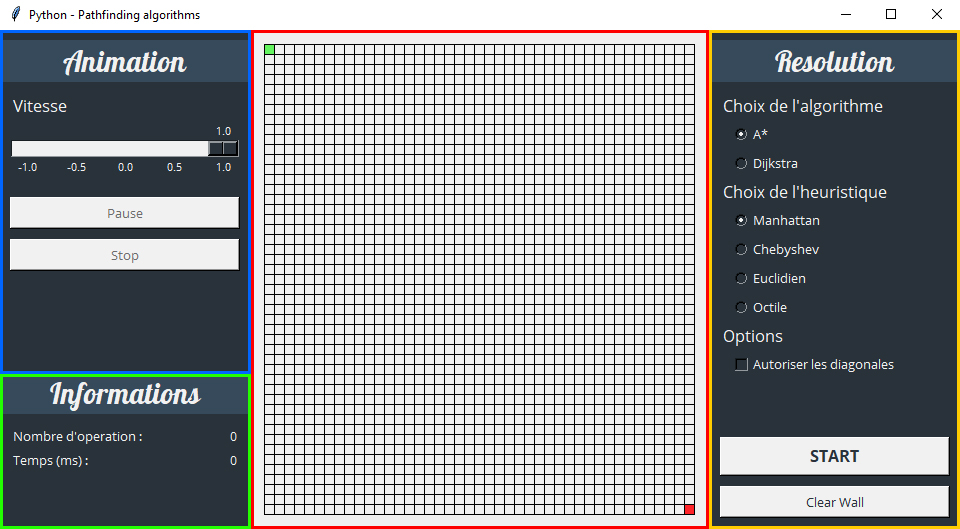
\includegraphics[scale=0.5]{UI.jpg}\\
		
		Comme nous pouvons le voir, l'interface se divise en 4 parties :
		\begin{itemize}
			\item[•] Le menu de gestion de l'animation
			\item[•] Le panneau d'affichage des informations
			\item[•] La grille éditable
			\item[•] Le menu du choix de l'algorithme et des options
		\end{itemize}
		
	\section{Grille}
	Afin d'avoir une grille dont l'édition soit aussi intuitive que possible, toute son ergonomie a été tournée autour du système de drag \& drop.
	Nous pouvons ainsi déplacer les cases de départ, d'arrivée et créer/supprimer des obstacles très simplement. \\\\
	Pour cela, l'implémentation de la grille sera divisé en 3 parties :
		\begin{itemize}
			\item[•] Les cellules
			\item[•] Les événements
			\item[•] La grille
		\end{itemize}
	\vspace{4mm}
	\vspace{4mm}
	Chaque cellule a 2 états possible :
		\begin{itemize}
			\item[•] vide : représente un déplacement possible
			\item[•] pleine : représente un obstacle
		\end{itemize}
	\vspace{4mm}
	Les événements permettrons d'interpréter les actions de l'utilisateur. \\
	Et enfin la grille permettra le liens entre tous ces éléments.
	
	\section{Menu}
		\subsection{Animation}
		L'ordinateur étant bien plus rapide que nous, si l'on impose pas de délai lors de l'animation, celle-ci serai instantané et perdrai tout son intérêt.\\
		Nous avons donc ajouté un curseur pour pouvoir régler la vitesse d'animation. Par ailleurs, une vitesse négative a également été autorisé afin de pouvoir remonter l'animation.
		Le réglage du délai d'attente va suivre une fonction de façon à ce que celui-ci soit plus fin lorsque l'on réduit la vitesse.
		
		\subsection{Résolution}
		Pour avoir le choix de l'algorithme, de l'heuristique et des options que l'on doit utilisé pour la résolution, le menu de résolution sera composé de 3 éléments : 2 listes de boutons radio et des cases à cocher pour les options.
		Un bouton pour supprimer tous les obstacles de la grille a également été ajouté par simple soucis d'ergonomie.\\\\
		Lorsque l'on clique sur le bouton "Start", alors la résolution se lance :
			\begin{enumerate}
				\item Activation des boutons pour l'animation
				\item Récupération des choix de l'utilisateur
				\item Récupération de la position des cases de départ / d'arrivée
				\item Lancement de l'algorithme choisi
				\item Lancement de l'animation si une solution a été trouvé, sinon affichage d'un message d'erreur
			\end{enumerate}
	
	\section{Informations}
	Un des objectifs de cette implémentation étant le but pédagogique, l'affichage de certaines informations est important pour avoir des éléments de comparaison entre les différents algorithmes / heuristiques.
	Actuellement, 2 informations sont récupérées : le temps d'exécution, et le nombre d'opérations.
	Chaque information est récupérée depuis l'historique des actions, et affiché lors du déroulement de l'animation finale.
	
	\section{Configuration}
	Afin de pouvoir personnaliser l'interface facilement, un fichier de configuration a été mis en place.
	Que ce soit les couleurs, les polices d'écriture, ou les dimensions des différents éléments qui composent l'interface, 
	une variable statique y est associé.
	
\chapter*{Conclusion}
\addcontentsline{toc}{chapter}{Conclusion}
De nombreuses améliorations sont encore possible, comme par exemple :
	\begin{itemize}
		\item[•] Pouvoir changer les dimensions de la grille a partir d'une fenêtre modale ou de la molette de la souris.
		\item[•] Pouvoir changer la résolution de la fenêtre au démarrage
		\item[•] Supporter l'ajout d'obstacle en cours de résolution (nécessite l'animation en temps réel)
	\end{itemize}
Cependant, au final, on se rend compte que l'algorithme ne fait pas tout. 
En effet, même si l'algorithme A* semble plus performant, il dépend encore de l'heuristique que l'on choisi. 
De plus, même le choix de l'heuristique change la charge de calcul, et donc le temps de résolution, mais plus important encore, la grille sur laquelle on lance la résolution à un impact.


% Annexe
\bibliography{bibliographie}
\bibliographystyle{alpha}

\end{document}
